\documentclass[twoside,11pt]{article}

% Any additional packages needed should be included after jmlr2e.
% Note that jmlr2e.sty includes epsfig, amssymb, natbib and graphicx,
% and defines many common macros, such as 'proof' and 'example'.
%
% It also sets the bibliographystyle to plainnat; for more information on
% natbib citation styles, see the natbib documentation, a copy of which
% is archived at http://www.jmlr.org/format/natbib.pdf

\usepackage{jmlr2e}
\usepackage{graphicx}
\graphicspath{ {images/} }



\begin{document}

\title{Research Paper: Machine Learning Application for Brain Tumor Localization in the  Repository of Molecular Brain Neoplasia Data (REMBRANDT) }

\maketitle
\textbf{Machine Learning for Health Care (Heinz 95-845) - Lukas Mohs}


\section{Abstract}
\noindent Within this paper, I want to present the putcome of the  combined application of \textit{Computer Vision} (CV) and  \textit{Machine Learning} (ML) to the \textit{Repository of Molecular Brain Neoplasia Data } (REMBRANDT) dataset. This dataset contains pre-surgical \textit{magnetic resonance} (MR) multi-sequence images of 130 patients. Based on a visual analysis and the application of several ML algorithms, I tried to predict the location of the brain tumor and compare it to the evaluation of three Radiologist, which defined the affected brain part and the potential impact on the brain functionality.i

\section{Introduction and Background}
\subsection{Brain Cancer}
Among all types of cancer, brain cancer is one of the deadliest even if it's not one of the most common ones. With a so-called \textit{5-Year Relative Survival Rate} of 32 \% for white people and 39 \% for black people it ranks on place 7 out of 26 for the lowest survival rate. Specific cancer types like \textit{Glioblastoma}, a very fast growing type of tumor, even has a a rate of 5\%. Especially in the later years of life, this rate decreases heavily for all types of brain cancer. \citep{cite1}
The high variance in the surivial rate is given by many factors such as the type of tumor, the location and of course whether it was treated. Especially the latter ones formed a major part of scientific studies that included ways of scanning the human brain for malignant tissue as well as the way of stopping the growth of the tumor cells. \citep{cite2}


\subsection{Magnetic Resonance Imaging (MRI)}
\textit{Magnetic Resonance Imaging} (MRI) addressed the challange of 
\textit{scanning} the human body by using \textit{radiology}  to see different layers of the inner tissue or organs. These different layers can be combined together to construct a 3-dimensional model of any part of the body. Mainly a strong  \textit{magnetic fields} is used in combination with \textit{radio waves}  and so-called \textit{field gradients}.
In comparison to \textit{Computer Tomography} (CT), MRI doesn't rely on \textit{X-radiation}, which qualifies it as a less harmful method. It should be mentioned that the magnetic waves of MRI can affect \textit{cardiac pacemakers} so that exceptions apply. \citep{edelman1993magnetic}

\subsection{The Human Brain}
Especially the development and refinement of the MRI technology favored advanced studies about the structure and functionality of the human brain. In order to understand the classification task of the presented algorithm, the major parts of the human brain are shortly described:
\begin{figure}{\textwidth}
	\centering
	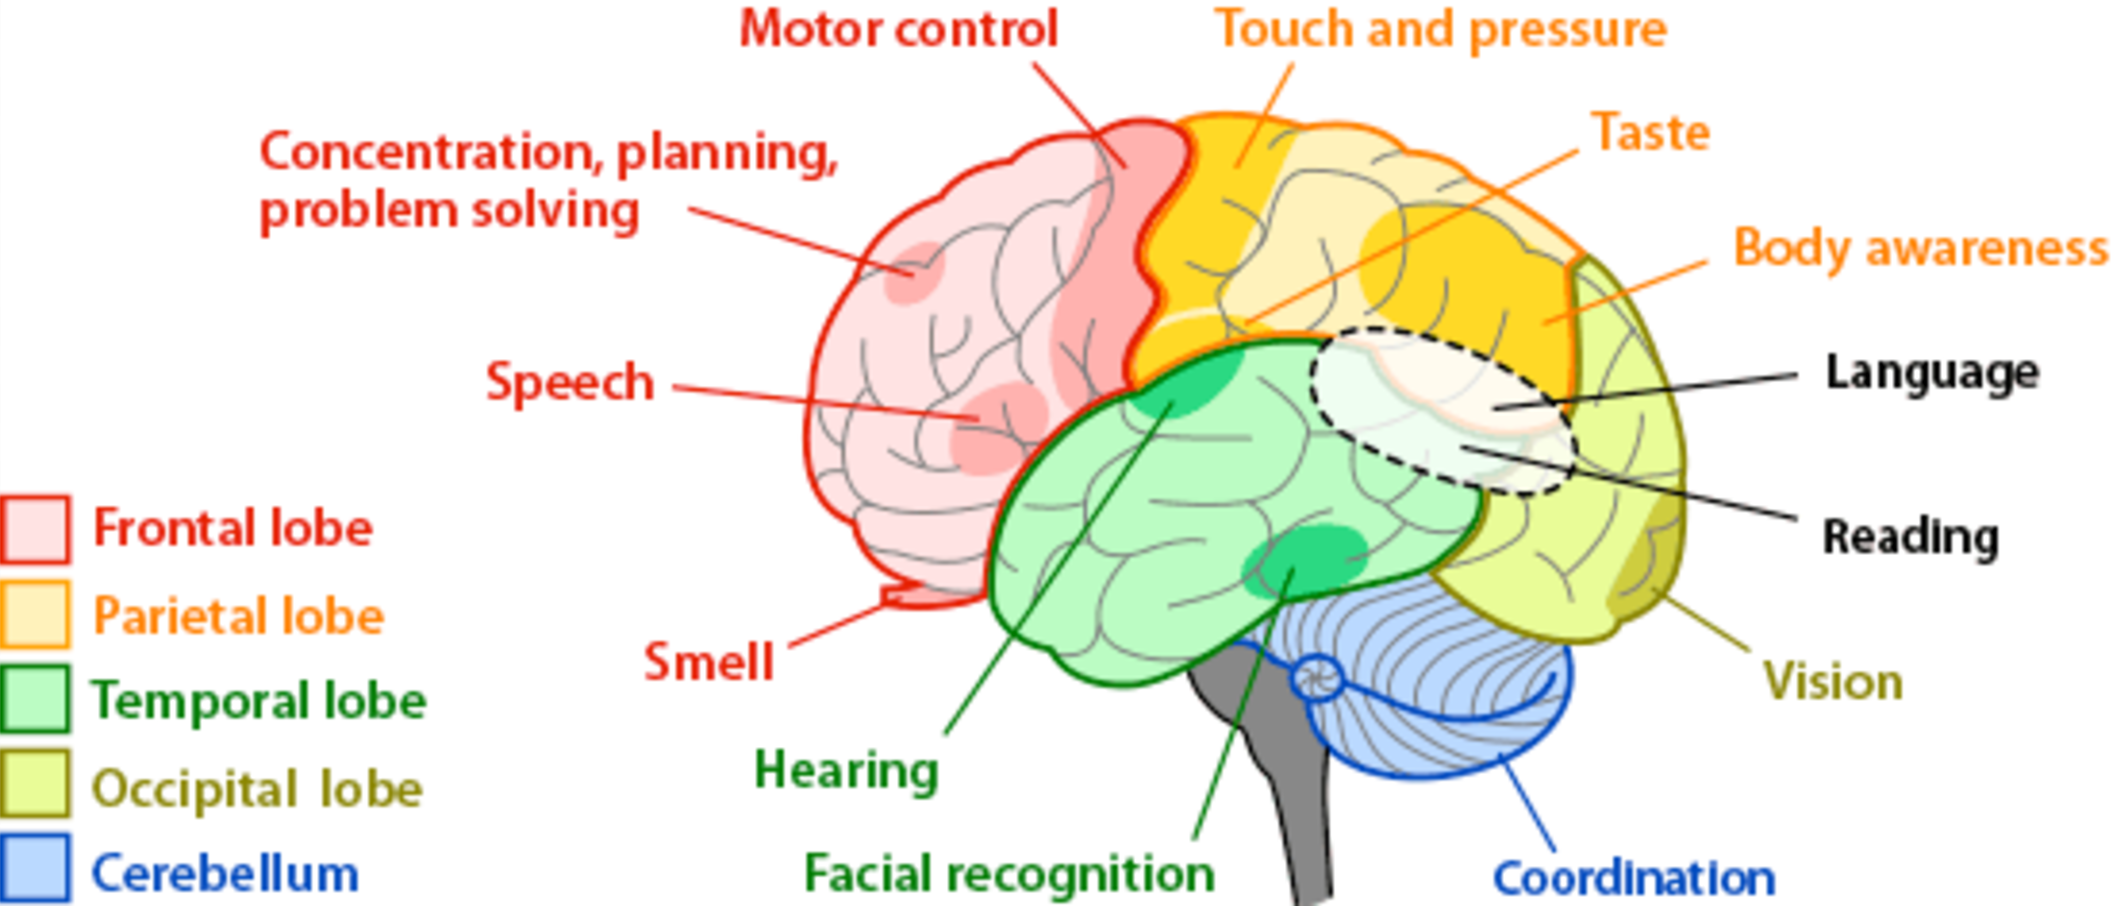
\includegraphics[width=10cm]{brain-areas}
	\caption{Brain Areas (source: Arizona State University)}
\end{figure}%

\begin{itemize}
	\item \textit{Frontal Lobe:} resides in the front of the head and is the only lobe on the lateral surface and separated from the other ones. It is responsible for problem solving, planning but also processes stimuli from the nose. 
	\item \textit{Temporal Lobe:} caudally joins the parietal and occipital lobe without a clear boundary. Researchers could show that it hosts the function of recognizing faces.
	\item \textit{Parietal Lobe:} is Clear separated from frontal lobe but merges into temporal and occipital lobe. It is important for the control of the body including the sense of touch.
	\item \textit{Occipital Lobe:} has also no clear coundary to its neighbours (parietal and temporal lobe). The stimuli of the eye are for example processed by this lobe.
	\item \textit{The Insula:} is a small portion of the cerebral cortex and hidden by the other outer lobes. It is believed to be responsible for  consciousness.
	\item \textit{The Cerebellum:} is placed on the back of the head below the occipital lobe and next to the \textit{brain stem}. It could be shown that it is responsible for fine motoric controls and languages.
\end{itemize}
\citep{duvernoy2012human}

\subsection{Computer Vision}
\textit{Computer Vision} (CV) is a field of \textit{Computer Science} that focusses on the way of how to digitally process, analyze and understand images. Driven by the development of cheap cameras and computing power, CV is applied in many cirsumstances to support or replace the human's richest sense: the eye.
To provide a highlevel understanding of a CV identification or classification approach, one has to consider the digital representation of an image on the computer. This can be decomposed to a two-dimensional matrix, where each entry holds a tupel of three values: the \textit{\textbf{R}ed}, \textit{\textbf{G}reen} and \textit{\textbf{B}lue} (RGB) channel. This tupel identifies how the color of one specific \textit{pixel} is composed. These matrix of pixels is often referred to as \textit{raster graphic}. Figure \ref{fig:pixel} demonstrates this representation for three specific pixels within an image. Most common file types represent these three channel values  in a range between 0 and 255. The brightness of an image is therefore determined by the average of the sum of each pixel's RGB values. The contrast of an image is referring to the variance of the sum of each pixel's RGB values: the higher the difference, the stronger the contrast. These concepts are important to later understand the image processing algorithm.

\begin{figure}{\textwidth}
	\label{fig:pixel}
	\centering
	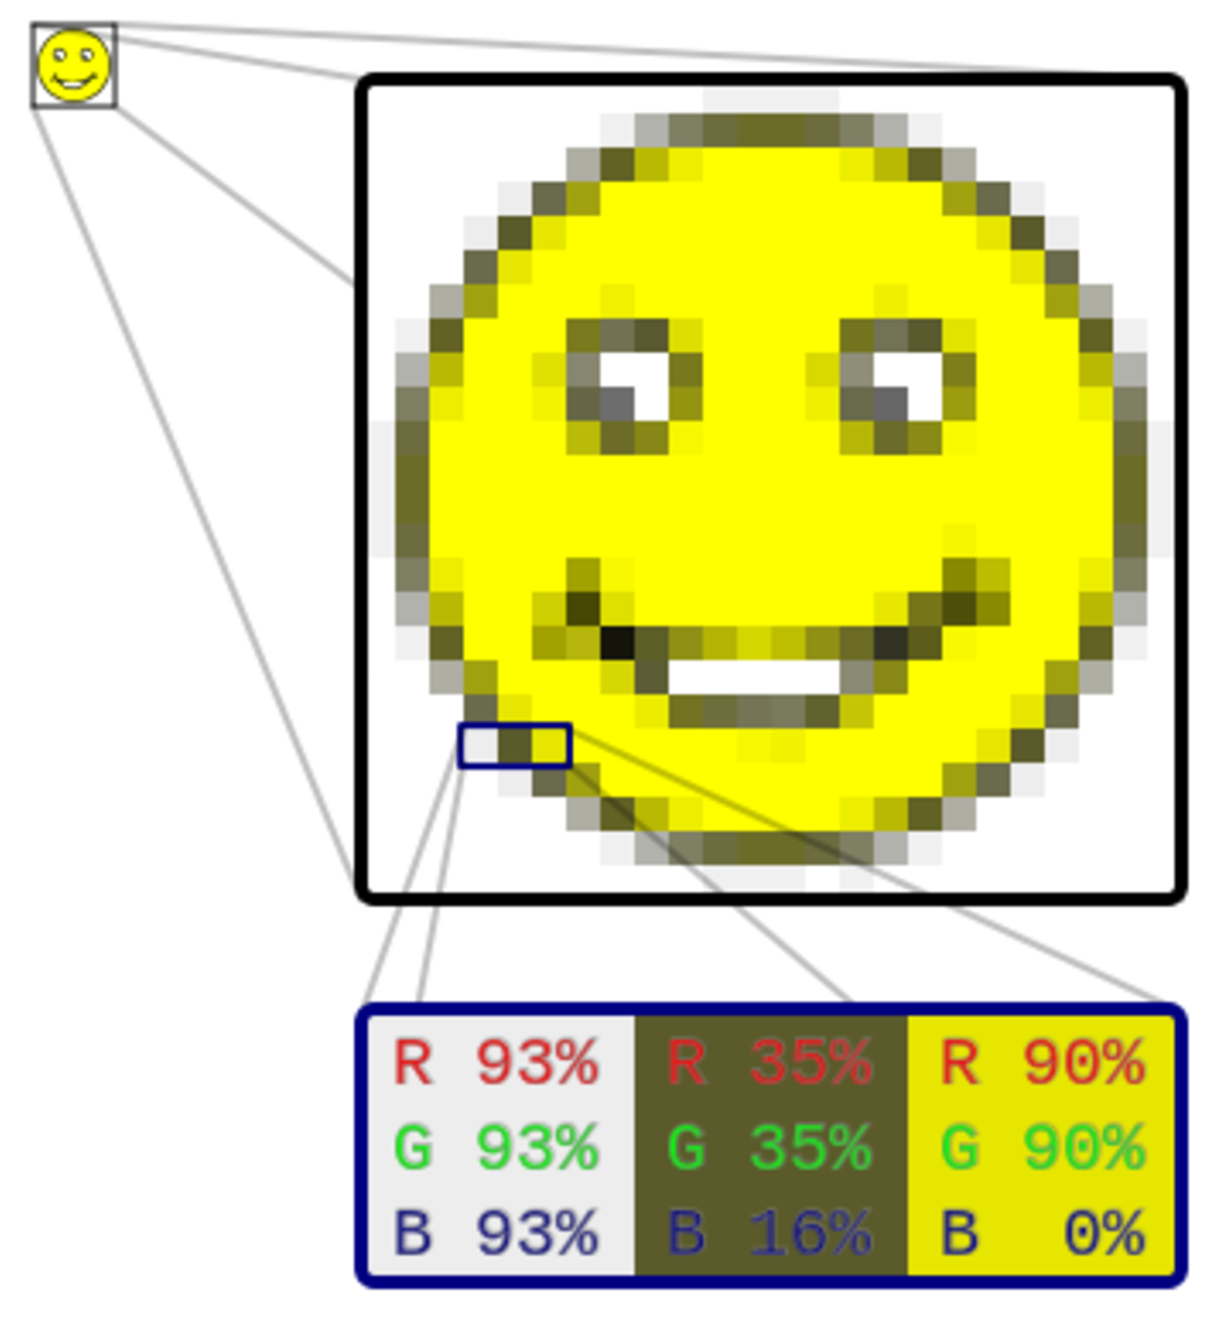
\includegraphics[height=5cm]{pixel}
	\caption{Raster Graphics (source: Wikipedia)}
\end{figure}%

\subsection{Machine Learning}
In the recent years, \textit{Machine Learning} (ML) genereated special attention due to it's successful application in many fields of industry. Generally, ML can be understood as an automized approach of analyzing and learning specific patterns within a big series of data. For this purpose, statistical principles are implemented on a given \textit{training set} afterwards to predict the class or value of new instances. ML is used in this scenario to evaluate the output of the image processing step and locate the brain tumor within a given sequence of MRI scans. In particular, the probabilistic \textit{Naive Bayes} classifier will be used in combination with a \textit{Decision Tree} due to their simplicity, whcih allows a solid interpretabiliby.

\section{Implementation: ML Prediciton based on CV Pattern Matching Outcomes}
Within this section I want to describe the setup and implementation of the \textit{ensemble} of CV and ML that is used to locate the brain tumor within the image sequence retrieved from the MRI scan. Ensemble means that a two-step process is used to realize the final prediction:
\begin{itemize}
	\item First, the images fo the REMBRANDT dataset are retrieved, preprocessed and analyzed by the application of several pattern matching methods.
	\item Then, the output of the analysis is written to \textit{CSV} file to be taken as an input for the ML learning and prediction approach.
\end{itemize}

\subsection{REMBRANDT Image Data Set}
At this point, the input data in form of a series of image sequences is described: 
The data of REMBRANDT was generated through the Glioma Molecular Diagnostic Initiative and contains the pre-surgical MR multi-sequence images from 130 patients. Each sequence can be defined as one specifc direction of slicing, which was used in order to scan the patient's head. This means that each patient was scanned either  horizontally or vertically from different angles. In figure \ref{fig:sequences}, one image of each of these sequnces for one patient is provided.

\begin{figure}{\textwidth}
	\label{fig:sequences}
	\centering
	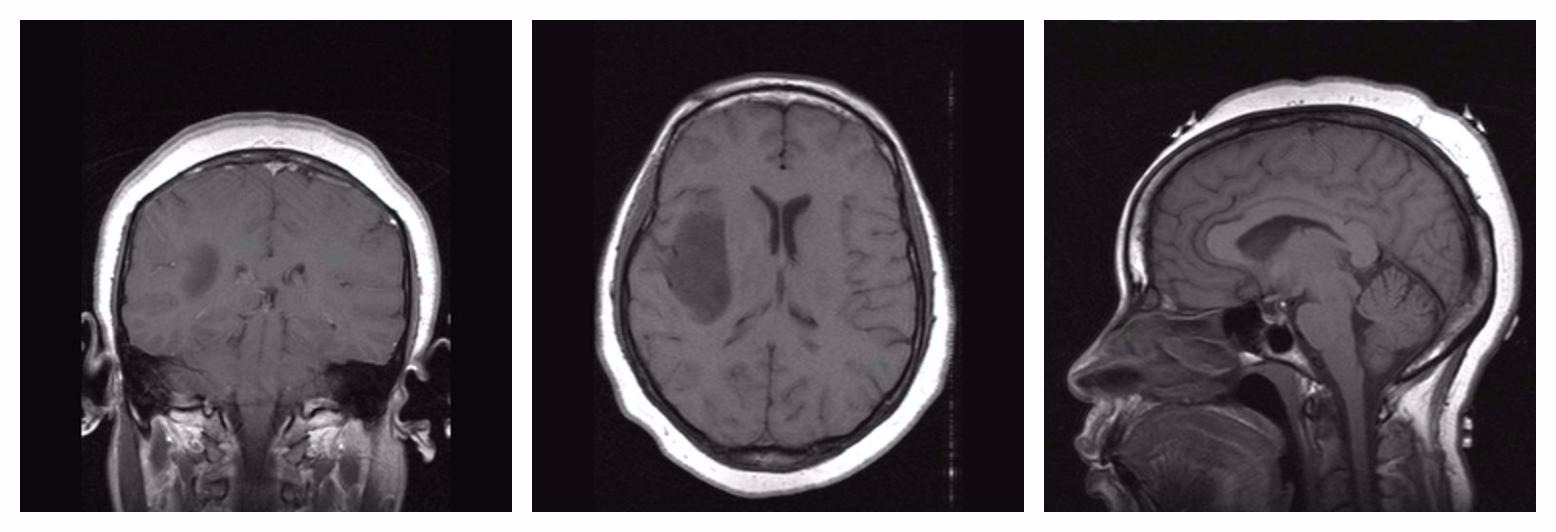
\includegraphics[height=5cm]{sequences}
	\caption{Sequence Comparison}
\end{figure}%


\bibliography{tumorDetection}
%\appendix
%\section*{Appendix A.}
%Some more details about those methods, so we can actually reproduce them.

\end{document}
